\subsection{Initial Results}
As described in Section~\ref{sec:proposed_approach}, we conducted a series of initial experiments to evaluate the performance of various machine learning models on the prediction of major oxide compositions from our \gls{libs} dataset.
These experiments aimed to provide a preliminary assessment of the models' performance.
All models were trained on the same preprocessed data using the Norm 3 preprocessing method described in Section~\ref{sec:norm3}.
This ensured that the models' performance could be evaluated under consistent and comparable conditions.

Table~\ref{tab:init_results} presents the results of these experiments, including the \gls{rmsep}, \gls{rmsecv}, standard deviation, standard deviation of cross-validation, and the mean of these metrics for each model and oxide.
Figure~\ref{fig:init_results_rmses} shows the mean \gls{rmsep} and \gls{rmsecv} for each model sorted in ascending order.

Notes on the results:
\begin{itemize}
    \item \textbf{Best performing models}: XGBoost, SVR and GBR perform the best.
    \item \textbf{Worst performing models}: Elastic Net, CNN and ANN perform the worst.
    \item \textbf{Oxide specific performance}: \ce{SiO2} and \ce{FeO_T} generally have higher \gls{rmsep} and \gls{rmsecv} values across most models, which is expected based on previous results. These oxides are known to be difficult to predict. On the other hand, \ce{MgO} and \ce{Na2O} have lower \gls{rmsep} and \gls{rmsecv} values across most models.
    \item \textbf{Mention mean values}: The mean values for RMSEP and RMSECV provide an overall performance indicator for each model. For example, XGBoost, GBR, and SVR have the lowest mean RMSEP and RMSECV values. The mean standard deviation values for these models are also lower - underscores reliability.
    \item \textbf{Relative performance}: Discuss this - mention that the jump between the three worst models is really high. Use this as an argument to justify the exclusion of these models from further experiments.
\end{itemize}

\begin{figure*}[h]
    \centering
    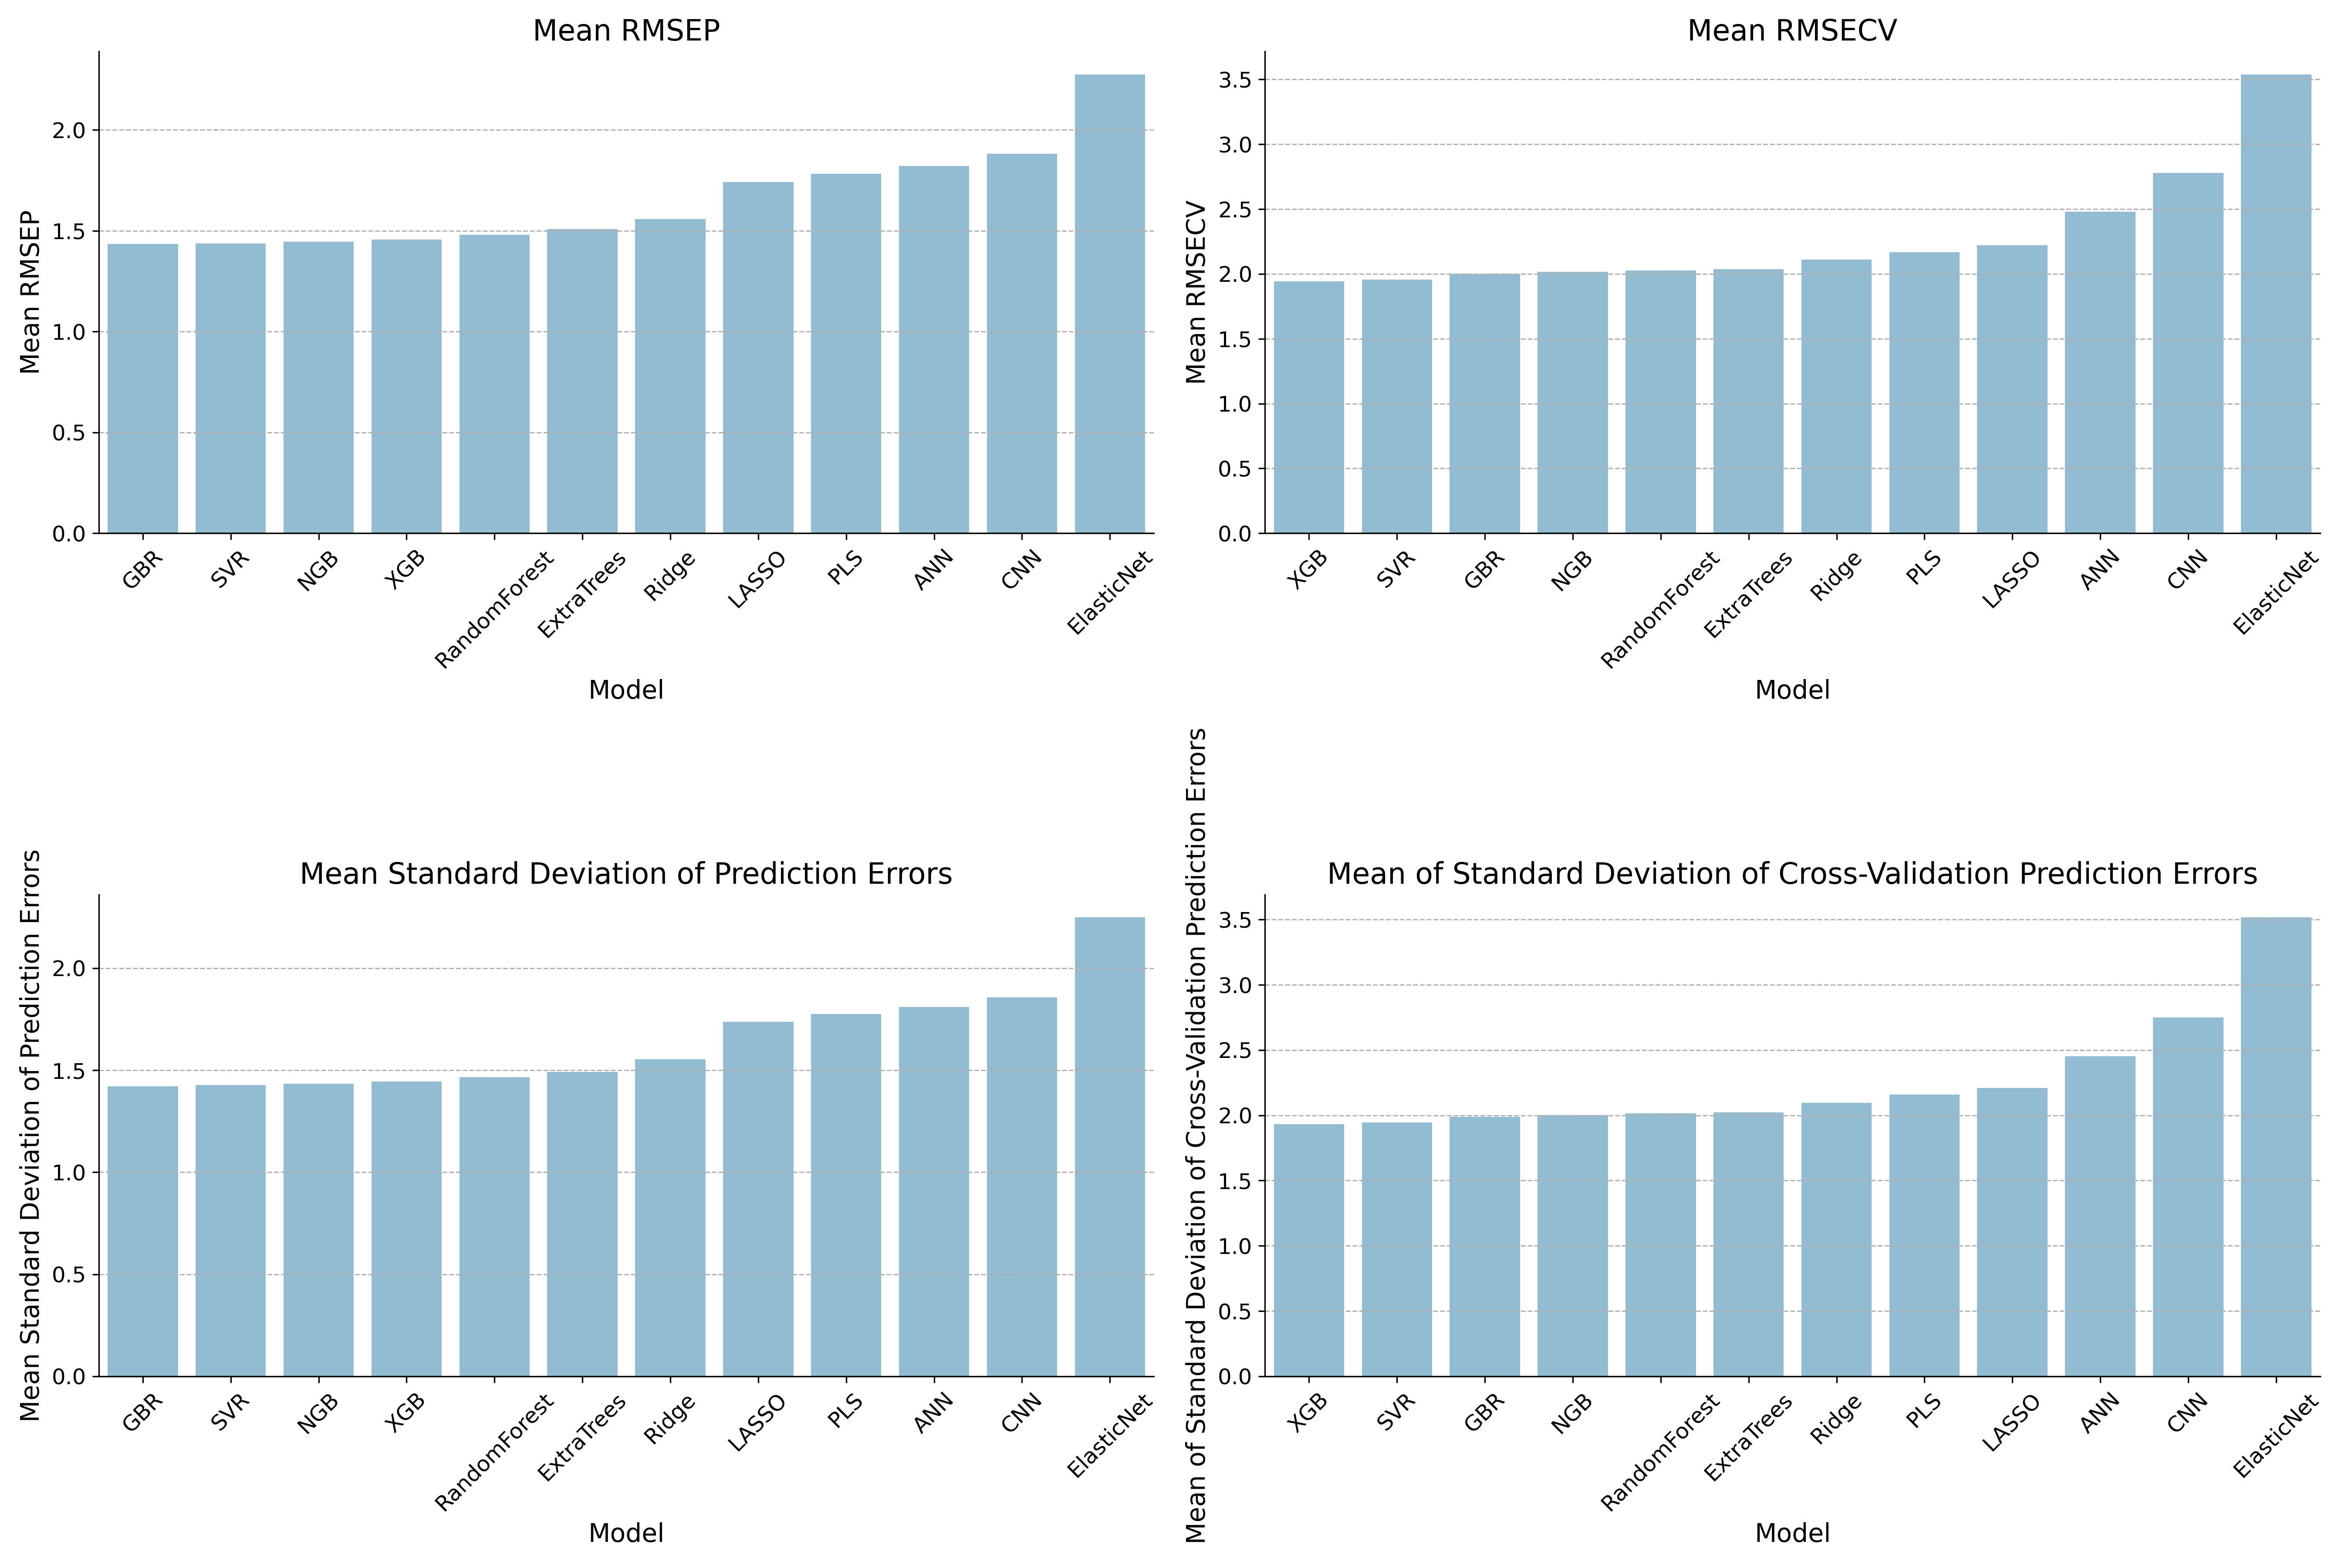
\includegraphics[width=\textwidth]{images/init_results_means.png}
    \caption{Mean \gls{rmsep}, \gls{rmsecv}, standard deviation of prediction errors, and standard deviation of cross-validation prediction errors for each model across all oxides.}
    \label{fig:init_results_rmses}
\end{figure*}

\begin{table}[ht]
\centering
\begin{tabularx}{\linewidth}{lrr}
\toprule
Model & Relative Performance (\%) & Diff. vs Next (\%) \\
\midrule
\gls{xgboost} & 100.00 & 0.85 \\
\gls{svr} & 100.85 & 2.22 \\
\gls{gbr} & 103.07 & 0.87 \\
\gls{ngboost} & 103.94 & 0.51 \\
\gls{rf} & 104.45 & 0.39 \\
\gls{etr} & 104.84 & 3.89 \\
Ridge & 108.74 & 2.92 \\
\gls{pls} & 111.66 & 2.73 \\
\gls{lasso} & 114.38 & 13.44 \\
\gls{ann} & 127.82 & 15.36 \\
\gls{cnn} & 143.18 & 39.18 \\
\gls{enet} & 182.36 & - \\
\bottomrule
\end{tabularx}
\caption{Relative performance of each model compared to the best performing model, and the difference in performance compared to the next best model.}
\label{tab:relative_performance}
\end{table}

\begin{table*}[]
\centering
\caption{Initial results for the different models and metrics.}
\resizebox{1\textwidth}{!}{%
\begin{tabular}{l|cccc|cccc|cccc}
Model & \multicolumn{4}{c}{Ridge} & \multicolumn{4}{c}{\gls{lasso}} & \multicolumn{4}{c}{\gls{enet}} \\
Metric & \multicolumn{1}{c}{RMSEP} & \multicolumn{1}{c}{RMSECV} & \multicolumn{1}{c}{Std. dev.} & \multicolumn{1}{c}{Std. dev. CV} & \multicolumn{1}{c}{RMSEP} & \multicolumn{1}{c}{RMSECV} & \multicolumn{1}{c}{Std. dev.} & \multicolumn{1}{c}{Std. dev. CV} & \multicolumn{1}{c}{RMSEP} & \multicolumn{1}{c}{RMSECV} & \multicolumn{1}{c}{Std. dev.} & \multicolumn{1}{c}{Std. dev. CV} \\
\hline
$\ce{SiO2}$ & 4.104 & 5.004 & 4.108 & 5.005 & 4.412 & 5.431 & 4.417 & 5.437 & 4.412 & 5.431 & 4.417 & 5.437 \\
$\ce{TiO2}$ & 0.424 & 0.470 & 0.413 & 0.469 & 0.398 & 0.556 & 0.389 & 0.555 & 0.398 & 0.556 & 0.389 & 0.555 \\
$\ce{Al2O3}$ & 2.322 & 2.913 & 2.324 & 2.888 & 2.349 & 3.063 & 2.352 & 3.044 & 2.349 & 3.063 & 2.352 & 3.044 \\
$\ce{FeOT}$ & 2.068 & 3.173 & 2.070 & 3.122 & 2.236 & 3.490 & 2.238 & 3.440 & 2.236 & 3.490 & 2.238 & 3.440 \\
$\ce{MgO}$ & 1.150 & 1.509 & 1.152 & 1.492 & 1.267 & 1.682 & 1.249 & 1.661 & 1.267 & 1.682 & 1.249 & 1.661 \\
$\ce{CaO}$ & 1.844 & 1.485 & 1.833 & 1.478 & 1.963 & 1.554 & 1.962 & 1.549 & 1.963 & 1.554 & 1.962 & 1.549 \\
$\ce{Na2O}$ & 0.632 & 1.089 & 0.633 & 1.084 & 0.625 & 1.114 & 0.616 & 1.111 & 0.588 & 1.085 & 0.587 & 1.082 \\
$\ce{K2O}$ & 0.651 & 0.668 & 0.645 & 0.668 & 0.638 & 0.859 & 0.629 & 0.856 & 0.638 & 0.859 & 0.629 & 0.856 \\
\hline
Mean & 1.649 & 2.039 & 1.647 & 2.026 & 1.736 & 2.219 & 1.732 & 2.207 & 1.731 & 2.215 & 1.728 & 2.203 \\
\hline
Model & \multicolumn{4}{c}{\gls{pls}} & \multicolumn{4}{c}{\gls{svr}} & \multicolumn{4}{c}{\gls{rf}} \\
Metric & \multicolumn{1}{c}{RMSEP} & \multicolumn{1}{c}{RMSECV} & \multicolumn{1}{c}{Std. dev.} & \multicolumn{1}{c}{Std. dev. CV} & \multicolumn{1}{c}{RMSEP} & \multicolumn{1}{c}{RMSECV} & \multicolumn{1}{c}{Std. dev.} & \multicolumn{1}{c}{Std. dev. CV} & \multicolumn{1}{c}{RMSEP} & \multicolumn{1}{c}{RMSECV} & \multicolumn{1}{c}{Std. dev.} & \multicolumn{1}{c}{Std. dev. CV} \\
\hline
$\ce{SiO2}$ & 4.141 & 5.701 & 4.145 & 5.693 & 3.552 & 4.908 & 3.555 & 4.908 & 3.715 & 5.304 & 3.699 & 5.292 \\
$\ce{TiO2}$ & 0.452 & 0.531 & 0.441 & 0.530 & 0.461 & 0.463 & 0.455 & 0.462 & 0.331 & 0.427 & 0.321 & 0.425 \\
$\ce{Al2O3}$ & 2.073 & 3.322 & 2.061 & 3.302 & 1.931 & 2.700 & 1.934 & 2.693 & 2.076 & 2.443 & 2.079 & 2.433 \\
$\ce{FeOT}$ & 3.222 & 3.117 & 3.221 & 3.114 & 1.823 & 2.847 & 1.814 & 2.809 & 2.091 & 3.091 & 2.073 & 3.053 \\
$\ce{MgO}$ & 1.106 & 1.296 & 1.103 & 1.296 & 0.789 & 1.426 & 0.785 & 1.419 & 0.911 & 1.742 & 0.904 & 1.731 \\
$\ce{CaO}$ & 1.937 & 1.813 & 1.923 & 1.792 & 1.626 & 1.532 & 1.594 & 1.508 & 1.765 & 1.503 & 1.754 & 1.499 \\
$\ce{Na2O}$ & 0.545 & 0.908 & 0.536 & 0.906 & 0.742 & 1.096 & 0.725 & 1.086 & 0.420 & 1.028 & 0.421 & 1.023 \\
$\ce{K2O}$ & 0.774 & 0.650 & 0.772 & 0.646 & 0.567 & 0.690 & 0.555 & 0.689 & 0.524 & 0.681 & 0.476 & 0.676 \\
\hline
Mean & 1.781 & 2.167 & 1.775 & 2.160 & 1.436 & 1.958 & 1.427 & 1.947 & 1.479 & 2.027 & 1.466 & 2.017 \\
\hline
Model & \multicolumn{4}{c}{\gls{ngboost}} & \multicolumn{4}{c}{\gls{gbr}} & \multicolumn{4}{c}{\gls{xgboost}} \\
Metric & \multicolumn{1}{c}{RMSEP} & \multicolumn{1}{c}{RMSECV} & \multicolumn{1}{c}{Std. dev.} & \multicolumn{1}{c}{Std. dev. CV} & \multicolumn{1}{c}{RMSEP} & \multicolumn{1}{c}{RMSECV} & \multicolumn{1}{c}{Std. dev.} & \multicolumn{1}{c}{Std. dev. CV} & \multicolumn{1}{c}{RMSEP} & \multicolumn{1}{c}{RMSECV} & \multicolumn{1}{c}{Std. dev.} & \multicolumn{1}{c}{Std. dev. CV} \\
\hline
$\ce{SiO2}$ & 4.112 & 5.071 & 4.081 & 5.010 & 3.576 & 4.995 & 3.479 & 4.922 & 3.953 & 4.898 & 3.926 & 4.876 \\
$\ce{TiO2}$ & 0.340 & 0.433 & 0.333 & 0.430 & 0.474 & 0.449 & 0.473 & 0.446 & 0.334 & 0.437 & 0.328 & 0.436 \\
$\ce{Al2O3}$ & 1.931 & 2.291 & 1.933 & 2.282 & 1.894 & 2.518 & 1.891 & 2.511 & 1.912 & 2.198 & 1.913 & 2.193 \\
$\ce{FeOT}$ & 1.588 & 3.561 & 1.590 & 3.530 & 1.594 & 3.069 & 1.596 & 3.068 & 1.848 & 3.020 & 1.838 & 3.002 \\
$\ce{MgO}$ & 0.849 & 1.578 & 0.845 & 1.574 & 0.964 & 1.766 & 0.960 & 1.763 & 0.905 & 1.781 & 0.901 & 1.771 \\
$\ce{CaO}$ & 1.740 & 1.610 & 1.723 & 1.602 & 1.768 & 1.468 & 1.769 & 1.468 & 1.765 & 1.467 & 1.749 & 1.457 \\
$\ce{Na2O}$ & 0.416 & 0.921 & 0.415 & 0.916 & 0.481 & 1.130 & 0.481 & 1.123 & 0.387 & 1.071 & 0.387 & 1.062 \\
$\ce{K2O}$ & 0.582 & 0.675 & 0.545 & 0.673 & 0.727 & 0.609 & 0.719 & 0.610 & 0.547 & 0.658 & 0.511 & 0.657 \\
\hline
Mean & 1.445 & 2.017 & 1.433 & 2.002 & 1.435 & 2.001 & 1.421 & 1.989 & 1.456 & 1.941 & 1.444 & 1.932 \\
\hline
Model & \multicolumn{4}{c}{\gls{etr}} & \multicolumn{4}{c}{\gls{ann}} & \multicolumn{4}{c}{\gls{cnn}} \\
Metric & \multicolumn{1}{c}{RMSEP} & \multicolumn{1}{c}{RMSECV} & \multicolumn{1}{c}{Std. dev.} & \multicolumn{1}{c}{Std. dev. CV} & \multicolumn{1}{c}{RMSEP} & \multicolumn{1}{c}{RMSECV} & \multicolumn{1}{c}{Std. dev.} & \multicolumn{1}{c}{Std. dev. CV} & \multicolumn{1}{c}{RMSEP} & \multicolumn{1}{c}{RMSECV} & \multicolumn{1}{c}{Std. dev.} & \multicolumn{1}{c}{Std. dev. CV} \\
\hline
$\ce{SiO2}$ & 3.995 & 5.230 & 3.970 & 5.225 & 4.664 & 7.025 & 4.670 & 6.981 & 4.662 & 6.061 & 4.626 & 6.046 \\
$\ce{TiO2}$ & 0.330 & 0.439 & 0.321 & 0.438 & 0.436 & 0.543 & 0.431 & 0.540 & 0.571 & 0.634 & 0.565 & 0.628 \\
$\ce{Al2O3}$ & 1.845 & 2.368 & 1.847 & 2.359 & 2.624 & 3.049 & 2.628 & 3.026 & 2.482 & 2.871 & 2.457 & 2.854 \\
$\ce{FeOT}$ & 2.144 & 3.299 & 2.126 & 3.257 & 2.534 & 3.836 & 2.497 & 3.748 & 2.588 & 4.584 & 2.521 & 4.488 \\
$\ce{MgO}$ & 0.906 & 1.755 & 0.895 & 1.738 & 1.315 & 1.818 & 1.300 & 1.768 & 1.292 & 2.892 & 1.280 & 2.857 \\
$\ce{CaO}$ & 1.837 & 1.515 & 1.831 & 1.510 & 1.799 & 1.633 & 1.772 & 1.634 & 2.009 & 2.142 & 2.008 & 2.099 \\
$\ce{Na2O}$ & 0.411 & 1.031 & 0.409 & 1.028 & 0.539 & 1.095 & 0.532 & 1.091 & 0.656 & 1.364 & 0.657 & 1.357 \\
$\ce{K2O}$ & 0.591 & 0.642 & 0.540 & 0.636 & 0.659 & 0.850 & 0.640 & 0.845 & 0.783 & 1.684 & 0.742 & 1.657 \\
\hline
Mean & 1.507 & 2.035 & 1.492 & 2.024 & 1.821 & 2.481 & 1.809 & 2.454 & 1.880 & 2.779 & 1.857 & 2.748 \\
\hline
\end{tabular}%
}
\label{tab:init_results}
\end{table*}
